\documentclass[letterpaper, 10pt]{article}

%---- packages----------------------------%
\usepackage{geometry}
\usepackage{titling}
\usepackage{hyperref}
\usepackage{ulem}
\usepackage{booktabs}
\usepackage{siunitx}
\usepackage{graphicx}
\usepackage{amsmath}
\usepackage{siunitx}
\usepackage{natbib}
\usepackage{xurl}
\usepackage[labelfont=bf,labelsep=period]{caption}
%----------------------------------------------%


\renewcommand{\figurename}{Supporting Fig.}


\begin{document}

\setlength{\droptitle}{-8em} 
\title{\Large\textbf{\textit{Supporting Information}\vspace{1em} \\
Legacy of microbial composition matters in simulating climate-driven litter decomposition}\vspace{-0em}}
\author{\normalsize\textbf{Bin Wang\textsuperscript{1,2,*}, Steven D. Allison\textsuperscript{2,3}}
\vspace{1em}\\
Environmental Science Division, Oak Ridge National Laboratory \textsuperscript{1} \\
Departments of Ecology and Evolutionary Biology \textsuperscript{2} 
and of Earth System Science \textsuperscript{3}\\
University of California Irvine\vspace{1em} \\
*Correspondence: wbwenwu@gmail.com} 
%\date{\normalsize August, 2020\vspace{0em}}
\maketitle

This document serves to appendix the main text with parameterization of DEMENTpy, forcings across
the climate gradient in Southern California, and model formulation, supporting text and results, as structured
and detailed below:
\begin{enumerate}
\item DEMENTpy
\item Climate gradient, DEMENTpy forcings, and microbial communities
\item Supporting results
\end{enumerate}

%#############################################################################
\section{DEMENTpy}
\subsection{Bridging osmolytic production and drought tolerance}

\subsection{Dispersal}
Dispersal is a key process in microbiome assembly and functioning. DEMENTpy deals with
 dispersal explicitly with a few assumptions on environmental factors controlling 
 dispersal rate ($R_{d}$), which follows:

\begin{equation}
  R_{d} = ?? 
\end{equation}

%#############################################################################
\section{Climate gradient, DEMENTpy forcings, and microbial communities}
This document details the preparation for DEMENTpy inputs at each of 
 the five sites simulated across the climate gradient (\textbf{Figure 1}).
 In detail, inputs including water potential, soil temperature, and litter 
 chemistry were processed and derived. Water potential was derived from 
 precipitation via an intermediate step of converting the precipitation 
 data. Python code [in the format of Jupyter Notebook(.ipynb)] underlying
 all of the processing is accessible at a GitHub Repo (\url{https://github.com/bioatmosphere/microbiome-climate-gradient.git}).
 With step-by step demonstrations, those readers who have a
 keen interest are supposed to be able to easily reproduce these preparations.

% figure 1: location of the five sites
\begin{figure}[h]
\centering
  %\begin{center}
      \includegraphics[width=1.0\linewidth]{../figures/site_location.pdf}
      \caption{Location of the five sites across the gradient. Map source:stamen.}
      \label{fig: figure 1}
  %\end{center}
\end{figure}

\subsection{\large Ecosystems across the Southern California climate gradient}

% table of the basic features of the five sites 
\begin{table}[h!]
  \begin{center}
    \caption{Five sites across the climate gradient.}
    \label{tab: table1}
    \begin{tabular}{lccc}
      \toprule % <-- Toprule here
      \textbf{Site} & \textbf{Latitude} & \textbf{Longitude} & \textbf{Elevation}\\
      %$\alpha$ & $\beta$ & $\gamma$ \\
      \midrule % <-- Midrule here
      Desert       & 33.648 & -116.38 & 275\\
      Scrubland & 33.610 & -116.45 & 1280\\
      Grassland & 33.737 & -117.70 & 470\\
      Pine-Oak  & 33.683 & -116.77  & 1710\\
      Subalpine & 33.823 & -116.75  & 2250\\
      \bottomrule % <-- Bottomrule here
    \end{tabular}
  \end{center}
\end{table}

All five sites (\textbf{Table 1}) are located on granitic parent material and experience
 Mediterranean precipitation patterns (cool, wet winters; hot, dry summers). This climate 
 gradient covers a temperature range from ... to...



\subsection{\large Environmental Forcing}

% figure of water potential and temperature of the five sites
\begin{figure}[h]
\centering
      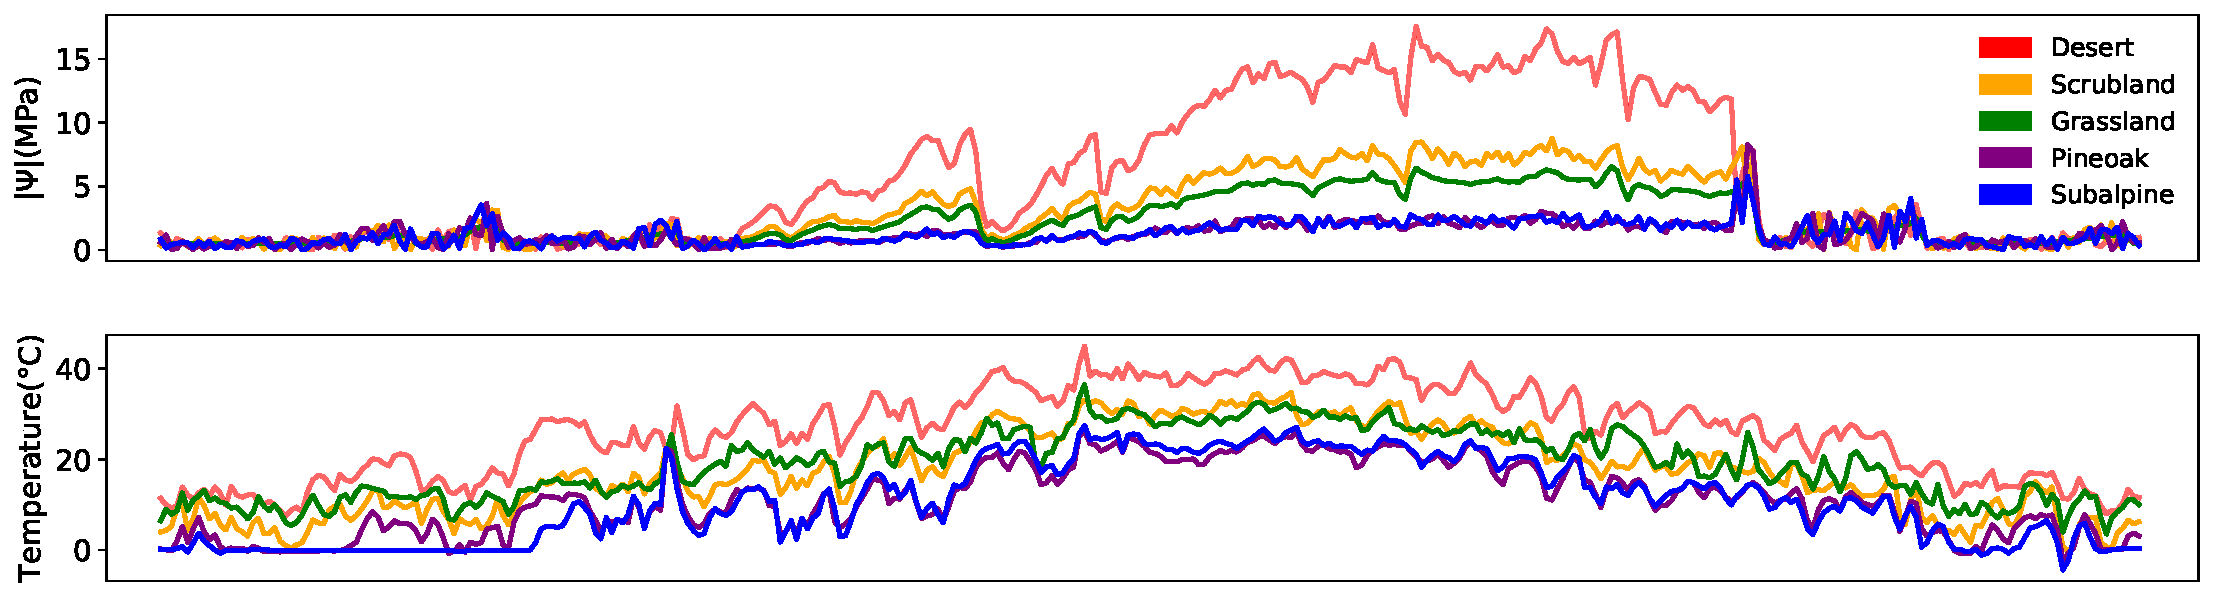
\includegraphics[width=1.0\linewidth]{../figures/gradient_forcing.pdf}
      \caption{\textbf{Forcings of the five sites across the gradient}. Note that the water potential is shown in absolute values.}
      \label{fig: figure 2}
\end{figure}

%~~~~~~~water potential~~~~~~~~
\subsubsection{Water Potential ($\psi$)}
As there are no leaf water potential ($\psi$; unit: MPa) across
the gradient readily available, a method of approximation was applied. Two approximation methods are developed based on
the only available, indirectly derived water potential data at the grassland site. With available measurements of water content ($\theta$; unit: g H\textsubscript{2}O g\textsuperscript{-1} wood) of grassland litter, daily water
potential was derived by \citet{allison2017consequences} at the grassland site
for a record of 3 years(2011-2013). This derivation of water potential followed a conversion
from water content to water potential as per the equation [\citet{dix1985changes}, referenced in \citet{allison2017consequences}]:

\begin{equation}
  \psi_{grassland} = -10^{0.118-0.114\log_{10} \theta}
\end{equation}

One way is extrapolating the other four sites from the grassland site by a simple scaling relationship. Water potential ($\psi_{site}$) of each of the other four sites was then derived by 
 linearly scaling grassland site water potential ($\psi_{grassland}$) with Total Annual Precipitation
 (\textbf{TAP}; unit: mm) and annual mean temperature at each site following:

\begin{equation}
  \psi_{site} = \frac{TAP_{site}}{TAP_{grassland}} \psi_{grassland}
\end{equation}
One condition that makes this approximate scaling legitimate is the same Mediterranean 
precipitation patterns across the climate gradient (cool, wet winters and hot, dry summers).
However, snowfall is not explicitly considered The derived water potential is further
smootheed to reduce noise. A detailed implementation of the derivation is presented
in the Jupyter Notebook \textbf{\texttt{precipitation\_v1.ipynb}}.

The alternative is a machine learning-based approach with a simple linear regression algorithm. A linear regression model of water potential as a function of precipitation and temperature is built from the grassland site data. This model is then used to obtain water potential for the 5 sites from 2017-2019.


\subsubsection{Temperature (\SI{}{\celsius})}
DEMENTpy is conceived using litter temperature at a daily resolution in principle. 
 In practice, soil surface temperature is used instead to approximate the litter 
 temperature. Soil temperature data at a sub-daily time step across the gradient at 
 each of five sites were measured. Details with regards to the measurement method, 
 pre-, and post-processing are documented in \citet{glassman2018decomposition}. 
 These data are openly accesible at \url{https://github.com/stevenallison/UCIClimateExperiment/tree/master/updatednames}.
 From these field measurements, daily soil temperature was 
 derived by averaging all (replicates?) measurements in each day, which was further smoothed.
 A step-by-step demonstration of this derivation is presented in the Jupyter Notebook
 \textbf{\texttt{soil\_temperature.ipynb}}.


\subsection{\large Litter Chemistry and Input}
DEMENTpy requires substrate-specific inputs in terms of C, N, and P (\textbf{Table xx}).
 \textbf{Phospholipids} (i.e.,OrgP1 in the model) are a key component of all cell membranes
 (\url{https://en.wikipedia.org/wiki/Phospholipid}). Though compound-specific stoichiometry
 is clear for determining concentration by element, substrate-specific concentration
 (($Sub_i$); unit: mg cm\textsuperscript{-3}) needs to be determined. This derivation followed:
\begin{equation}
  Sub_{s,i} = f_{s,i} Ts 
\end{equation}
where $s$ is one of the five sites, $i$ is one of the 10 substrates, $f_{s,i}$ is
 the percentage of substrate $i$ in site $s$, and $T_s$ is the total concentration of 
 initial substrates (C+N+P) in site $s$.  $f$ was informed by field measurements of 
 litter chemistry at each site as presented in \citet{baker2017extracellular}. $T$ was 
 assumed the same across sites. As per the observation by \citet{baker2017extracellular}, 
 standing litter pools are largest in the grassland and pine-oak site, reduced in the
 subalpine site, significantly reduced in the scrubland site, and negligible in the desert
 site. A detailed script implementing these processes is presented in the Jupyter Notebook 
 \textbf{\texttt{litter\_chemistry\_v1.ipynb}}.


\subsection{Microbial communities across the gradient}
Microbial systems after four years presented significant differences across the gradient
with respect to decomposition and community-level enzyme investment and drought tolerance.
Enzyme investment was different among the five sites ($P$ $<$ 0.05). However, the drought tolerance

composition (biomass):

traits:

decomposition:

\bibliographystyle{authordate1}
\bibliography{references}

%###################################
%~~~~~~~~~~~Results~~~~~~~~~~~~~~~~~~
%###################################
\section{Supporting Results}

% figure 3: communities across the gradient
\begin{figure}[h]
\centering
      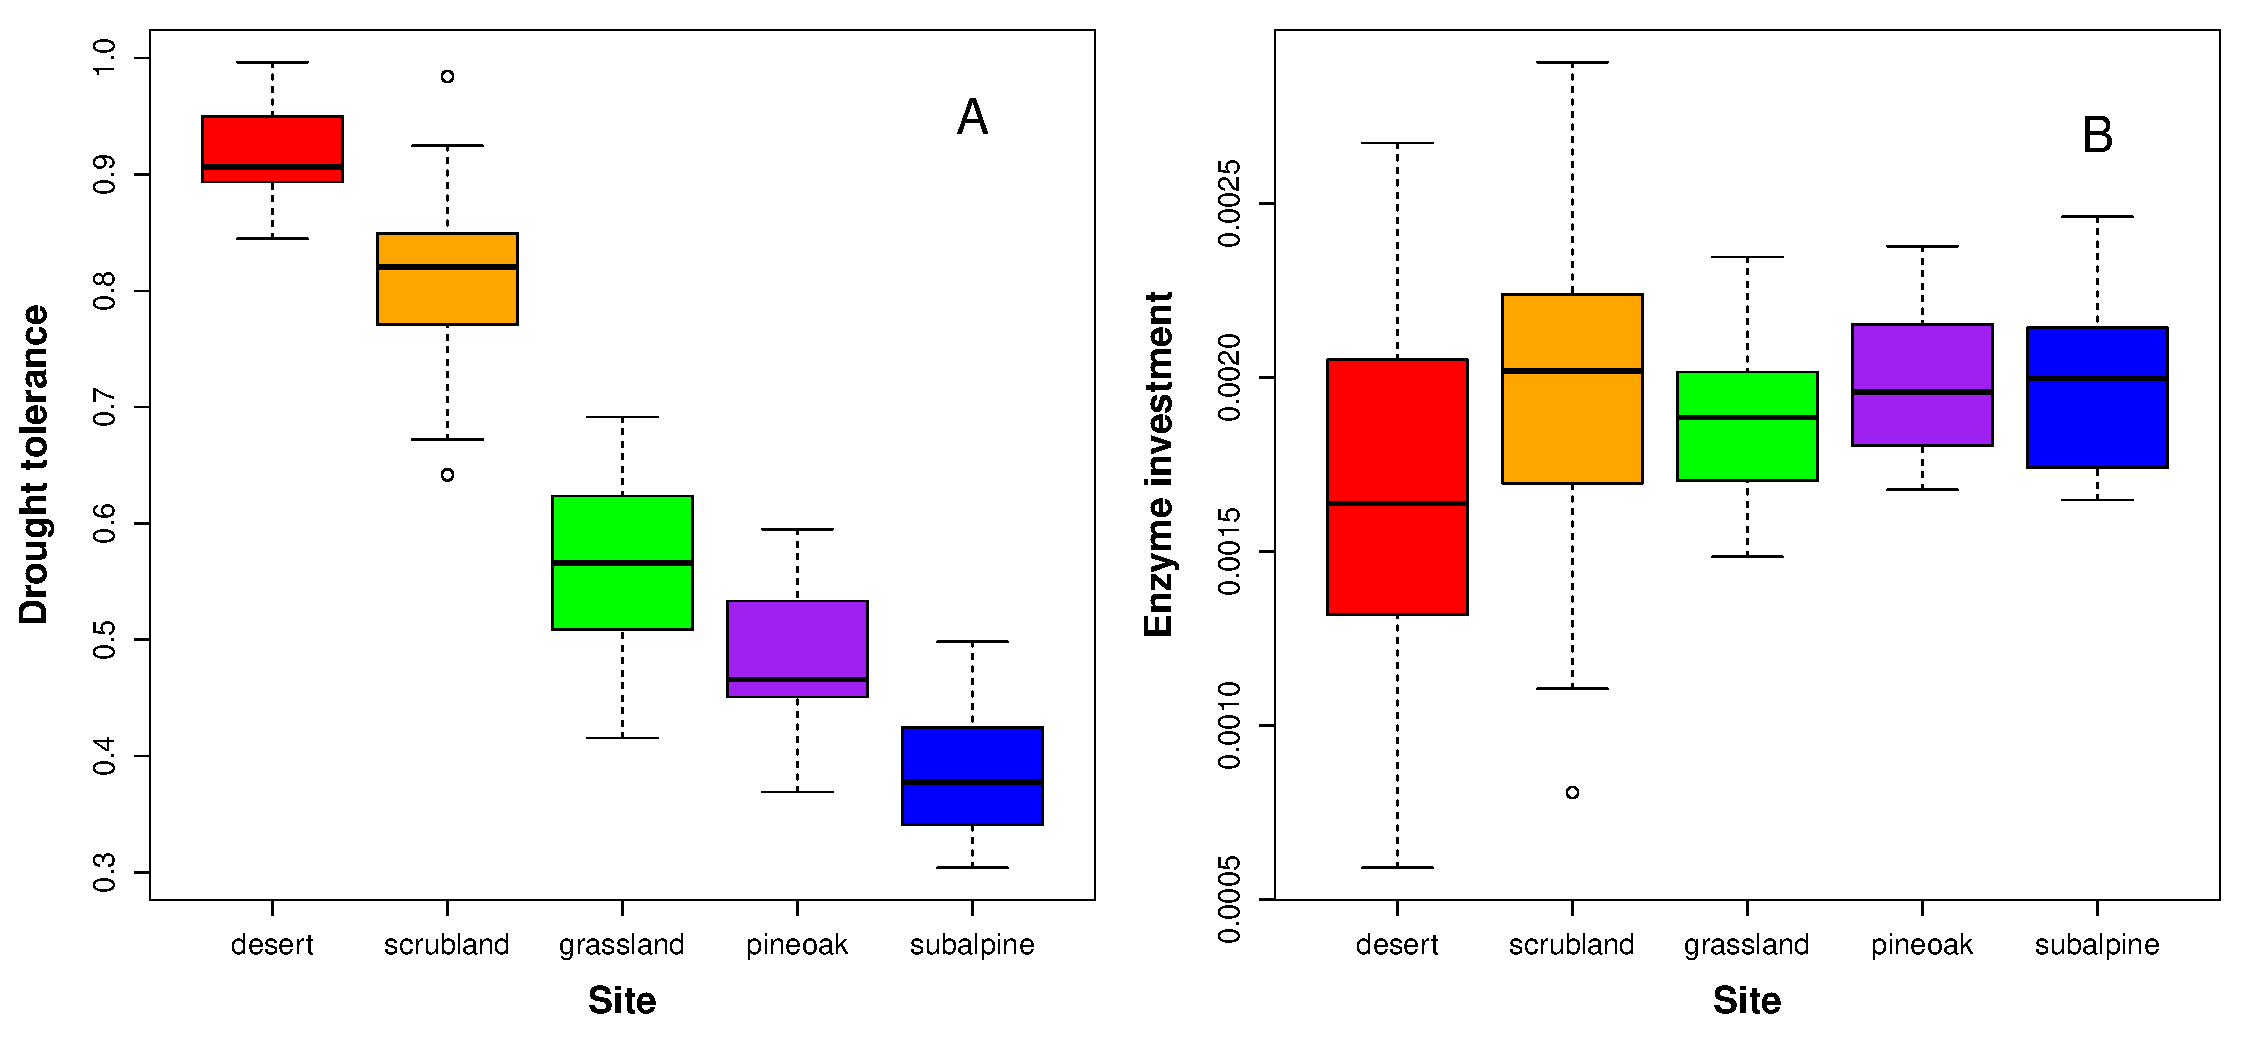
\includegraphics[width=1.0\linewidth]{../figures/community.pdf}
      \caption{\textbf{Community traits at the five sites across the gradient before transplant}.}
      \label{fig: figure 4}
\end{figure}


% figure 4: water potential and temperature of the five sites
\begin{figure}[h]
\centering
      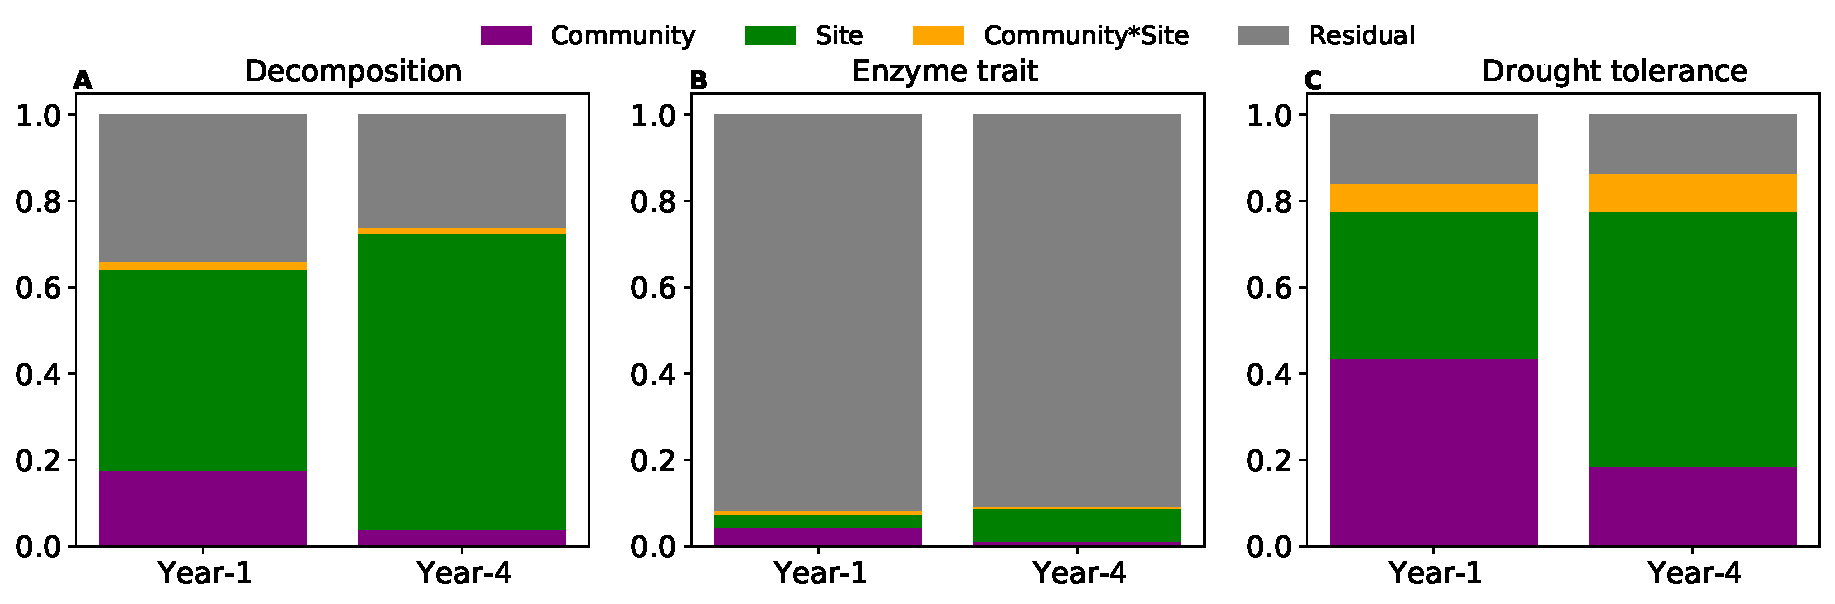
\includegraphics[width=1.0\linewidth]{../figures/relative_contribution.pdf}
      \caption{\textbf{Variance partitioning of decomposition (A), Enzyme trait (B), and
      Drought tolerance (C)}. Note in panel B only site and community are significant in year-1, and
      site significant in Year-4.}
      \label{fig: figure 4}
\end{figure}


% figure 5:
\begin{figure}[h]
\centering
      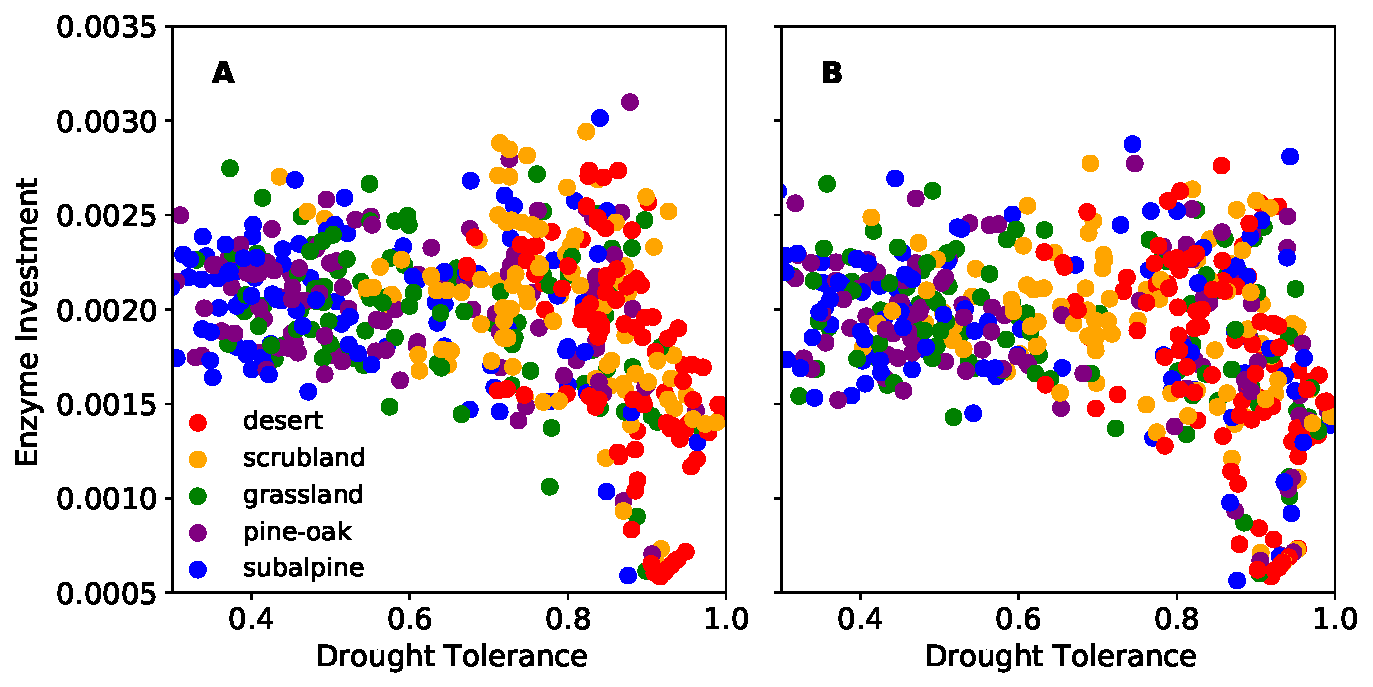
\includegraphics[width=1.0\linewidth]{../figures/pooled_trait_correlation.pdf}
      \caption{\textbf{Enzyme investment versus drought tolerance by the end of year 1 (A) and year 4 (B) after the transplant}. Data across the gradient were pooled together and colored by site.}
      \label{fig: figure 4}
\end{figure}


% figure 6: ternary plot
\begin{figure}[h]
\centering
      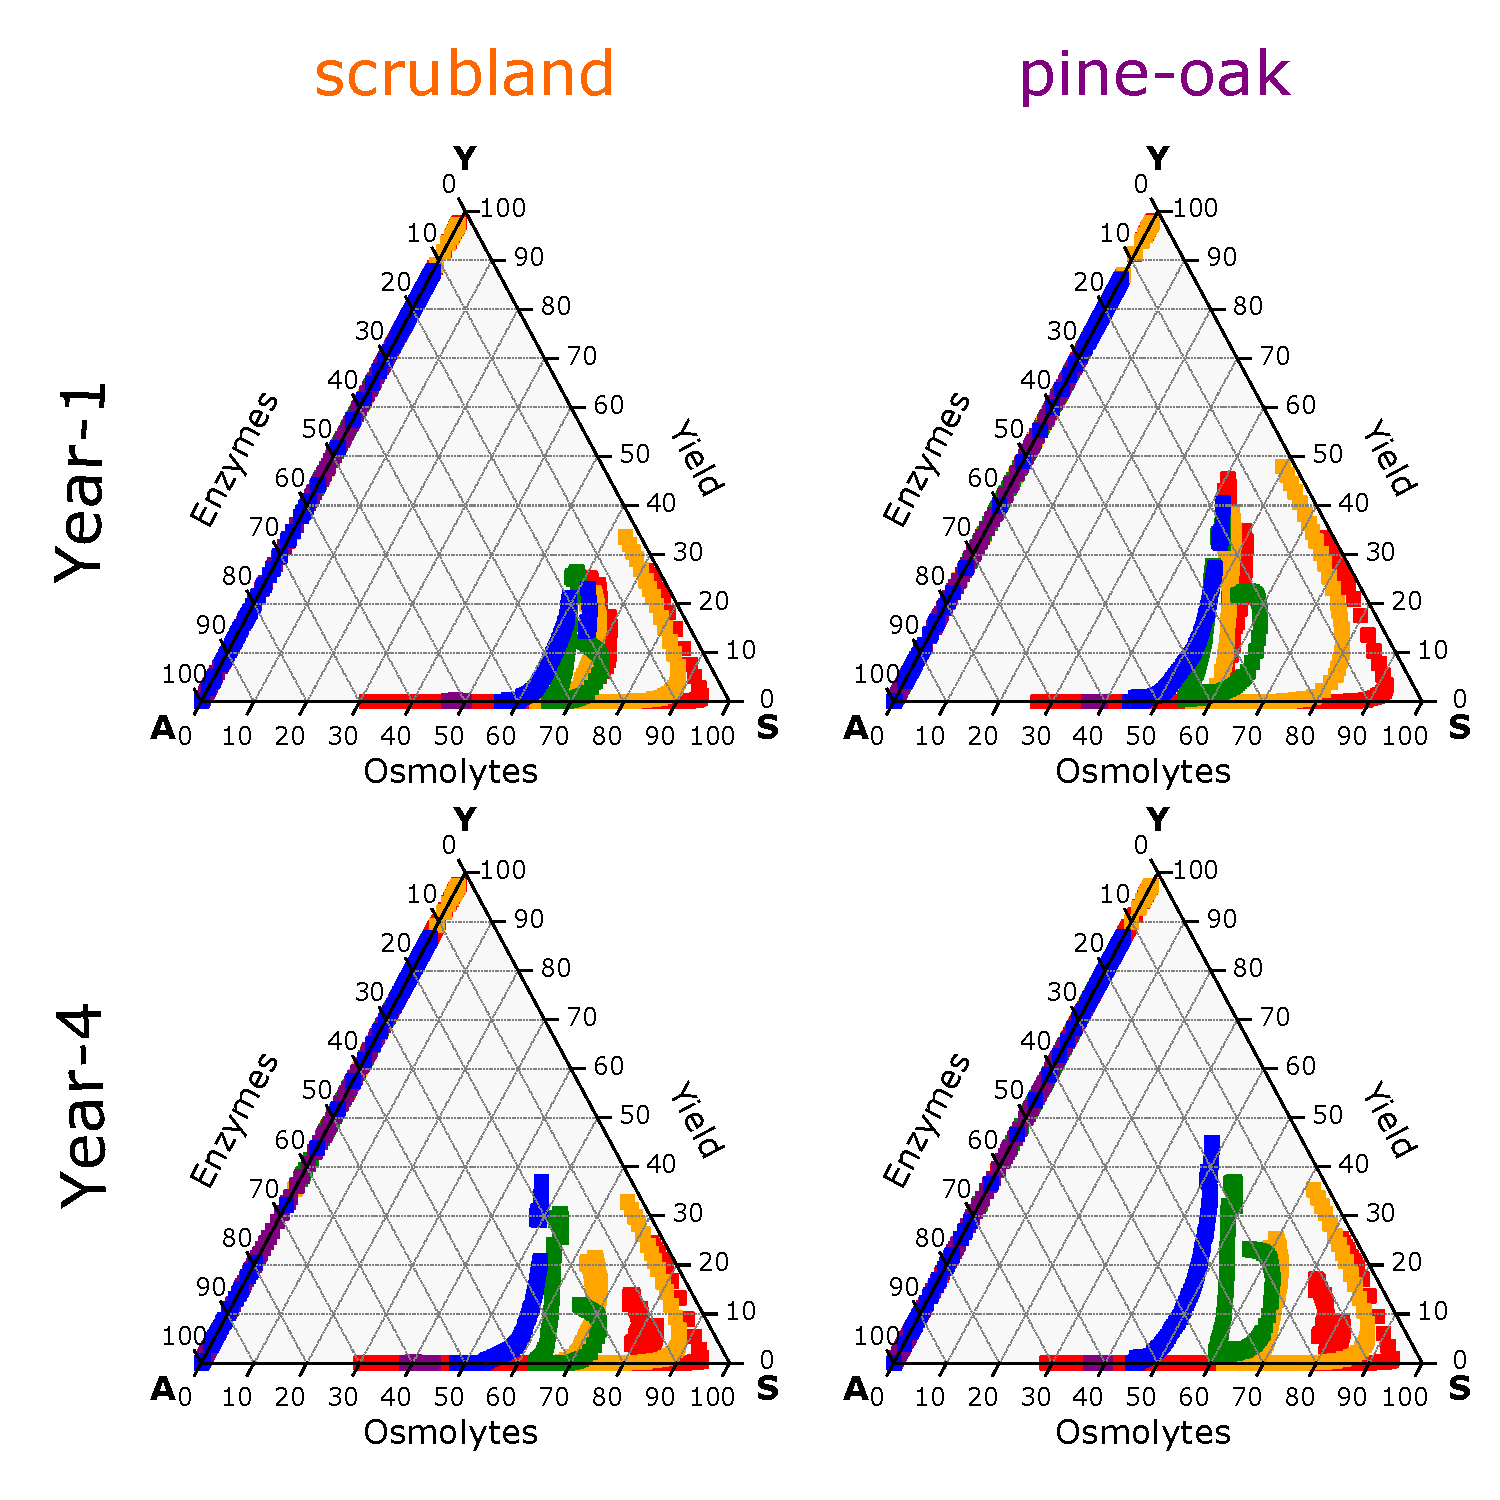
\includegraphics[width=1.0\linewidth]{../figures/ternary_2.pdf}
      \caption{\textbf{Ternary plots of allocation among enzyme, osmolyte, and yield}. Y, A, and S corresponding to Yield, Acquisition, and Stress tolerance}
      \label{fig: figure 3}
\end{figure}


\end{document}